% THIS IS SIGPROC-SP.TEX - VERSION 3.1
% WORKS WITH V3.2SP OF ACM_PROC_ARTICLE-SP.CLS
% APRIL 2009
%
% It is an example file showing how to use the 'acm_proc_article-sp.cls' V3.2SP
% LaTeX2e document class file for Conference Proceedings submissions.
% ----------------------------------------------------------------------------------------------------------------
% This .tex file (and associated .cls V3.2SP) *DOES NOT* produce:
%       1) The Permission Statement
%       2) The Conference (location) Info information
%       3) The Copyright Line with ACM data
%       4) Page numbering
% ---------------------------------------------------------------------------------------------------------------
% It is an example which *does* use the .bib file (from which the .bbl file
% is produced).
% REMEMBER HOWEVER: After having produced the .bbl file,
% and prior to final submission,
% you need to 'insert'  your .bbl file into your source .tex file so as to provide
% ONE 'self-contained' source file.
%
% Questions regarding SIGS should be sent to
% Adrienne Griscti ---> griscti@acm.org
%
% Questions/suggestions regarding the guidelines, .tex and .cls files, etc. to
% Gerald Murray ---> murray@hq.acm.org
%
% For tracking purposes - this is V3.1SP - APRIL 2009

\documentclass{acm_proc_article-sp}

\begin{document}

\title{SVM Approach to Automated Cardiac SPECT Diagnosis}
%
% You need the command \numberofauthors to handle the 'placement
% and alignment' of the authors beneath the title.
%
% For aesthetic reasons, we recommend 'three authors at a time'
% i.e. three 'name/affiliation blocks' be placed beneath the title.
%
% NOTE: You are NOT restricted in how many 'rows' of
% "name/affiliations" may appear. We just ask that you restrict
% the number of 'columns' to three.
%
% Because of the available 'opening page real-estate'
% we ask you to refrain from putting more than six authors
% (two rows with three columns) beneath the article title.
% More than six makes the first-page appear very cluttered indeed.
%
% Use the \alignauthor commands to handle the names
% and affiliations for an 'aesthetic maximum' of six authors.
% Add names, affiliations, addresses for
% the seventh etc. author(s) as the argument for the
% \additionalauthors command.
% These 'additional authors' will be output/set for you
% without further effort on your part as the last section in
% the body of your article BEFORE References or any Appendices.

\numberofauthors{4} %  in this sample file, there are a *total*
% of EIGHT authors. SIX appear on the 'first-page' (for formatting
% reasons) and the remaining two appear in the \additionalauthors section.
%
\author{
% You can go ahead and credit any number of authors here,
% e.g. one 'row of three' or two rows (consisting of one row of three
% and a second row of one, two or three).
%
% The command \alignauthor (no curly braces needed) should
% precede each author name, affiliation/snail-mail address and
% e-mail address. Additionally, tag each line of
% affiliation/address with \affaddr, and tag the
% e-mail address with \email.
%
% 1st. author
\alignauthor 
Dharmatheja Bhat\\
       \affaddr{SJCE, Mysore}\\
% 2nd. author
\alignauthor 
Supreeth Nag V.P.\\
       \affaddr{SJCE, Mysore}\\
% 3rd. author
\alignauthor
Varun B. Patil\\
       \affaddr{SJCE, Mysore}\\
% \and  % use '\and' if you need 'another row' of author names
% 4th. author
\alignauthor
Vinay M.\\
       \affaddr{SJCE, Mysore}\\
}
% There's nothing stopping you putting the seventh, eighth, etc.
% author on the opening page (as the 'third row') but we ask,
% for aesthetic reasons that you place these 'additional authors'
% in the \additional authors block, viz.
\date{15 June 2012}
% Just remember to make sure that the TOTAL number of authors
% is the number that will appear on the first page PLUS the
% number that will appear in the \additionalauthors section.

\maketitle
\begin{abstract}
This project aims to develop an automated system for detection of cardiac disease given pre-labelled SPECT (Single photon emission computed tomography) data to train the system and then provide it with unclassified SPECT data for the purpose of classification as indicating possible cardiac disease or not. For the purpose of this classification, we have used a well known and highly used Machine Learning classification algorithm known as Support Vector Machine. Popularly abbreviated as SVM, Support Vector Machines are a class of supervised machine learning algorithms meaning that in the training stage of the classifier, we provide the system with SPECT data pre-classified as indicating cardiac disease and not indicating cardiac disease. That is, you are teaching the system; the system is learning from the inputs you provide. Once the learning is complete, you can provide the system with SPECT data that has not been labelled and the system will classify them automatically for you. The accuracy of this classification will obviously depend on the the accuracy of the training set images, the parameters of the Support Vector Machine, the complexity of the training algorithm and many more factors which will be detailed later. This project has a lot of relevance in todays world especially when corporations are providing million dollar prize money to anyone who can build an automated system that can detect virtually any disease Star Wars style (a.k.a Transcoder) and improvements in machine learning is getting us closer to that goal.  
\end{abstract}

\keywords{SPECT, SVM, Support Vector Machines, aNN, Neural Networks, Linear Kernel, Gaussian Kernel} % NOT required for Proceedings

\newpage
\section{Introduction}

\subsection{Objective}

The objective of this project work is to build an automated system for automatically classifying SPECT heart data instances as possibly indicating a cardiac disease or not. The aim here is not to classify the type of cardiac disease if present.

\subsection{Existing Solution}

The existing solution is to have an experienced doctors trained eye and finely honed intuition recognize as possibly indicating a cardiac disease or not. Very few automated solutions exist, because they are not very accurate compared to an experienced human being and also because patients do not trust such systems with serious diseases relating to the heart. And it is not that a doctor is confronted with hundreds of patients with cardiac disease everyday. Thus, manually examining data is more efficient that spending considerable time and effort training an automated system that will be used only on a couple of patients a day.  

\subsection{Proposed Solution}

The proposed solution is to use state-of-the-art in machine learning to build an accurate classifier that can do the job of a doctor is deciding whether a particular instance of SPECT heart data indicated cardiac disease or not. Though it is not built to replace a highly paid cardiac specialist in hospitals anytime soon, the technology could well be used someday to dramatically reduce treatment costs and also improve accuracy of detection. We are actually moving closer to a day when the Star wars style handheld device (a.k.a Transcoder) which can detect any disease in an instant will become reality.

\subsection{Applications}

An automated classification system like the one we are building could be used by doctors as an auxiliary tool which can assist their finely honed skills. It can also be used to collect statistics from hospitals about cardiac diseases just from the instances of SPECT data instead of a doctor providing all the statistics which can be a laborious task and is un-necessary. Such an automated system can even one day be a part of a magic device that can help detect any disease. Most importantly information obtained from such a system can help less experienced doctors make informed decisions not that we are comfortable taking the opinion of a less experienced cardiologist.

\section{Using SVM for classification}

SVM short for Support Vector Machines is an important machine learning technique used mainly for classification of data. It is a supervised learning method meaning that the algorithm first needs to be provided with data that has already been classified. Using this, the algorithm learns parameters that correspond to the classification in the training data. Once training has been completed, the algorithm can then classify any other data which is called the test set instances.

\subsection{Tools Required}

The most important tool used to develop the program for this project is called Octave. Many people know it as an opensource alternative to Matlab. Apart from Octave being freely available and the core libraries occupying much less space than the Matlab software (which is a good thing for computers with limited disk space), it is known for being extremely efficient for numerical computations like the ones this project makes use of largely owing to expertly written numerical libraries for almost every advanced mathematical computation known to mankind. This saves you from re-inventing the wheel and also saves you a lot of time by allowing you to concentrate on refining the core concepts and not worry about the internal computations. But what makes Octave such a worthy alternative to Matlab is that it supports the exact same syntax as Matlab and can perform virtually anything you can do on Matlab in exactly the same way. Also, you will not need the bulk of the Matlab software to perform the computations for this project; the core libraries in Octave are more than sufficient. To install octave in Ubuntu, open up a terminal and type in the following command: 
\begin{displaymath}\text{\$ sudo apt-get install octave}\end{displaymath}

\subsection{Technologies Used}

This project implements an advanced machine learning algorithm known as Support Vector Machines (SVM) with Sequential Minimal Optimization as the learning algorithm. SVM's have the capability to produce high accuracy classifiers that are fast as well. Ofcourse, there are many variations in the parameters of the Support Vector Machine and the inputs that will ultimately decide the accuracy of the classifier. Nonetheless, Support Vector Machines are the state-of-the-art in supervised machine learning and is only fitting that such an important application is able to make use of it.

\subsection{Literature Dealing With The Topic}

The main literature behind the idea and implementation of this project is the paper titled ``Knowledge Discovery Approach to Automated Cardiac SPECT Diagnosis"\cite{KD}. This paper focusses on how data mining approaches can be used to mine for patterns in vast quantities of medical data to help professionals make informed decisions faster and also helps to discover new knowledge that would otherwise have gone unnoticed in the vast expanse of data. The writers claim that using highly optimized versions of Support Vector Machines can achieve the highest possible accuracy of all the other classification methods available. 

The paper titled ``Improving the Classification of Multiple Disorders using Problem Decomposition"\cite{CM} talks about using AIM Abductive Networks which is a supervised machine learning algorithms much like Support Vector Machines, but have an accuracy which is not very far from a well designed and highly tuned Support Vector Machine given that AIM abductive networks are substantially more complex than Support Vector Machines. The paper also hints about the GMDH type algorithms for Self-organizing methods in modelling which are advancements to Support Vector Machines (SVM).

A very recent paper titled ``Hierarchical Neural Networks for Partial Diagnosis in Medicine"\cite{HN} makes use of very advanced neural network models like inductive neural networks to achieve higher accuracy than our simple Support Vector Machine based classifier.

Of course there is one other class of algorithms that is widely used to solve problems in medicine. The paper titled ``Differential Diagnosis of diseases using Genetic Algorithms and Support Vector Machines" by Kim B.Y, Park K.S et al., gives a very broad overview of how Gentic algorithms can be used in conjunction with Support Vector Machines to help in computer-aided disease identification.

We have also looked at the following papers for a deeper and richer understanding of SPECT imaging and classification techniques -- ``Quantitative analysis in single photon emission tomography (SPECT)"\cite{QA}, ``A novel algorithm for classification of SPECT images of a human heart"\cite{NA}, ``Cardiac SPECT Imaging"\cite{CS}, ``Issues in Automating Cardiac SPECT Diagnosis"\cite{IS}, ``Analysing and improving the diagnosis of ischaemic heart disease with machine learning, Artificial Intelligence in Medicine"\cite{AI}, ``Diagnosing Myocardial Perfusion from SPECT Bulls-eye Maps - A Knowledge Discovery Approach"\cite{DM}.

\subsection{Supporting Systems}

The classifier is written in Octave and thus requires the GNU Octave software to be installed on the system. Note that, even though an Octave program looks very much like a Matlab program, an Octave program connot be executed on Matlab inside Windows.

\section{SVM Algorithm}

The SVM algorithm we are using is purely linear in its execution with the following sub-steps performed one after the other in a sequential manner.

\subsection{Inputs to the Algorithm}

SPECT is actually images. It has to be preprocessed to generate numerical data that the program can work on. SPECT images are few and far between. For all computational machine learning purposes, UCI maintains a comprehensive database of numerical SPECT data collected from some of the best medical institutions around the world that we will be using. The data set we will be using was obtained from http://archive.ics.uci.edu/ml/datasets/SPECT+Heart. 

The UCI data set is a comma-seperated-value file (CSV) which we read into the octave program as a two dimensional matrix using a built in function called csvread(). There are binary values for about 23 features indicating the presence or absence of a particular feature in that particular SPECT image instance. These features include left ventricular ejection fraction, stroke volume, myocardial perfusion, etc. 

The data is provided in two parts: ``Training set" used to train the machine learning classifier and ``Test set" used to test the classifiers accuracy. The Test Set itself is further divided into a Cross Validation set and a Test set. The CV consists of random samples from the Test Set. The cross validation(CV) set is primarily used to tune the classifier program for best performance; it is not used to gauge the accuracy of the classifier. For example, the CV set is used to select the best possible values for C and $\sigma$ used in the SVM algorithm. The remaining part of the Test Set is the one that is actually used to measure the accuracy of the classifier after it has been trained on the Training Set. 

Usually the data is divided as training set(60\%), CV set(20\%) and test set(20\%). The distribution between the sets is done randomly. Then, the hypothesis that minimizes the CV set error(fraction of CV set instances that are wrongly classified) is chosen and the error on the test set is reported as the generalized error.

\subsection{SVM Algorithm}

Our aim in designing the SVM algorithm was to find best relationship between the features and its class so as to minimize the error in classification. The algorithm we employ is called SMO(Sequential Minimal Optimization) and it finds the best possible class to which a particular instance of SPECT data belongs to. The term ``best class" here means the class which minimizes the classification error or likewise improves the classification accuracy. The two classes possible for any SPECT instance are: indicates possible cardiac disease, does not indicate cardiac disease(future enhancements to the project will include more fine grained classification or multiclass classification).

\subsection{Choices In Algorithm Design}

The SVM algorithm we have implemented can either use a Linear Kernel or a Gaussian Kernel. 

A Linear Kernel can be imagined to be a straight-line seperation between the classes(or a planar seperation in the case of multidimensional data). The Gaussian Kernel on the other hand can be visualized as a non-linear seperation between classed which also means a non-planar or curved seperation between classes of multidimensional data. Our implementation of the algorithm provides the option to switch the kernel on the fly meaning that the kernel can be changed for any particular execution of the algorithm. Now, the question arises as to which kernel to use, given that we have two choices.

\begin{equation}K_{linear}(x^i, x^j) = x^i * x^j\end{equation}
\begin{equation}K_{gaussian}(x^i, x^j) = \exp(-\frac{||x^i - x^j||^2}{2\sigma^2})\end{equation}

A Linear Kernel is usually employed when the number of features is more than the number of samples and a Gaussian Kernel is employed when the number of samples is more than the number of features. And also, the kernel used depends on whether the data itself is linearly-seperable or not.

\subsection{SVM Parameters}

We noted earlier that C and $\sigma$ are two important parameters that need to be decided by examining the Cross Validation set.

Informally, the C parameter is a positive value that controls the penalty for misclassified training examples. A large C parameter tells the SVM to try to classify all the examples correctly(large margin). However, large C means that it is more susceptible to outliers and does not give a natural fit for the data.

$\sigma$ is a parameter of the Gaussian Kernel which determines how fast the ``similarity measure" approaches 0 for data points that are further apart. If $\sigma$ is large, the similarity changes slowly and can cause underfitting. If $\sigma$ is small, the similarity changes fast and can cause overfitting.

In practice, C and $\sigma$ are selected from a set of highly possible values for both C and $\sigma$ where the values vary approximately by a factor of 10, by testing all possible combinations of C and $\sigma$ for the one that gives the least error in classification of the CV set. In our case we have the following set of values for C and $\sigma$ to choose from:

\begin{equation}C = [0.01, 0.03, 0.1, 0.3, 1, 3, 10, 30]\end{equation}
\begin{equation}\sigma = [0.01, 0.03, 0.1, 0.3, 1, 3, 10, 30]\end{equation}

\subsection{Optimization Problem in SVM}

The optimization problem in SVM is that of minimizing the following equation:

\begin{equation}J = (C * A) + B\end{equation}

where,

\begin{equation}A = \Sigma(y^i * cost_{1}(z)  +  (1-y^i) * cost_{0}(z))\end{equation}    
\begin{equation}B = \frac{1}{2} \Sigma(\Theta^2)\end{equation}
\begin{equation}cost_{1}(z) = -\log(z)\end{equation}
\begin{equation}cost_{0}(z) = -\log(1 - z)\end{equation}

Once we know $\Theta$, we can predict the class as follows:

\begin{equation}if(\Theta^Tx) > 0, \text{predict class} = 1\end{equation}
\begin{equation}if(\Theta^Tx) < 0, \text{predict class} = 0\end{equation}

\subsection{Outputs}

When all is said and done, we expect the classifier to tell you the class to which a particular SPECT instance belongs to. One way to check whether what the classifier predicts is ``upto the mark" is to compare the result with already known values. There are several ways to gauge this ``upto the mark" notion in terms of numerical values.

Prediction Accuracy is the fraction of the instances in the Test set that are correctly classified. Sensitivity is the fraction of positive instances in the Test Set that are correctly classified as belonging to the positive class. Specificity is the fraction of negative instances in the Test Set that are correctly classified as belonging to the negative class.

\begin{equation}\text{Accuracy} = \frac{\text{Test set instances correctly classified}}{\text{total Test set instances}}\end{equation}
\begin{equation}\text{Sensitivity} = \frac{\text{positive instances correctly classified}}{\text{total postive instances in Test set}}\end{equation}
\begin{equation}\text{Specificity} = \frac{\text{negative instances correctly classified}}{\text{total negative instances in Test set}}\end{equation}

When you have high values for all of the above numerical measures, you know that your classifier is ``upto the mark".

\section{Alternative Designs}

One of the most important alternative designs that we have prototyped prior to our full scale implementation of the SVM classifier is the aNN (artificial neural networks) version of the classifier because of its comparable complexity to the
SVM algorithm.

The first thing we observed with the neural networks prototype is that its accuracy heavily depends on its structure which is almost decided on ``intuition" alone. However, machine learning experts will testify to the fact that trusting your intuition is not a good idea. The upshot is that a neural network structure that seems perfect for one problem might perform terribly on another problem. It is just not possible to stick to one structure.

On the contrary, SVM does not rely on ``intuition". It is able to decide on the best parameters using information from the problem itself. In our case, the best possible values for C and $\sigma$ were determined from the problem itself(CV set).

Ofcourse several advanced algorithms can perform better and faster, but our goal has been to demonstrate the use of machine learning and data mining to improve and ease disease diagnosis and not designing the ultimate cardiologist substitute.

\section{Comparitive Studies}

\begin{figure}
\centering
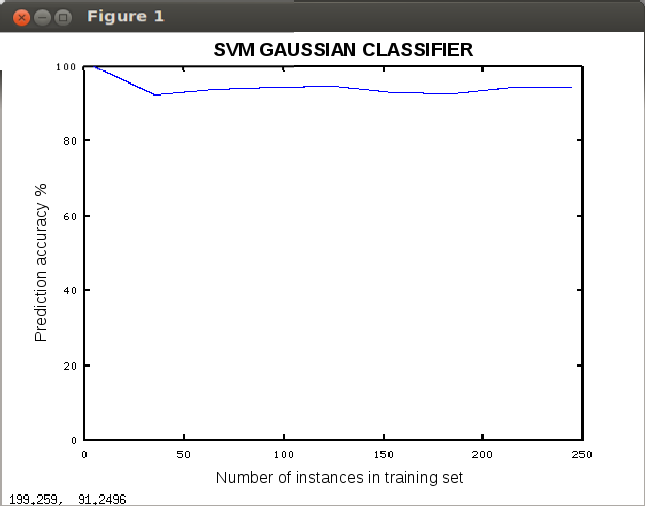
\includegraphics[width=2.5in, height=2.5in]{svmg.png}
\caption{SVM(gaussian kernel) accuracy}
\end{figure}
Figure 1 below shows the prediction accuracy for the SVM implementation using a non-linear (also called Gaussian) kernel. We can see that the accuracy is a constantly above 90\%. One important thing to notice that the accuracy is almost 100\% for a small number of instances. This is an idiosyncrasy in the data set. The data set consists of a huge number of samples that belong to class 1 (i.e, heart disease present), whereas there are very few examples in the data set that correspond to class 0 (heart disease not present), and hence when only a few instances are considered, it will most likely contain only instances that belong to class 1 and no instances that belong to class 0 which explains the reported accuracy of 100\%. This is not a true indication of the accuracy of the classifier. The true accuracy only becomes evident for a large number of training samples. Another thing to notice is that the graph is not smooth, rather it is spikey. The reason for this is that the accuracy is measured for an increase in number of instances by 30. This is because, if the graph was plotted in Octave for an increase in the number of instances of 1, it would take an unimaginably long amount of time to run through the algorithm with a total of close to 300 instances.

\begin{figure}
\centering
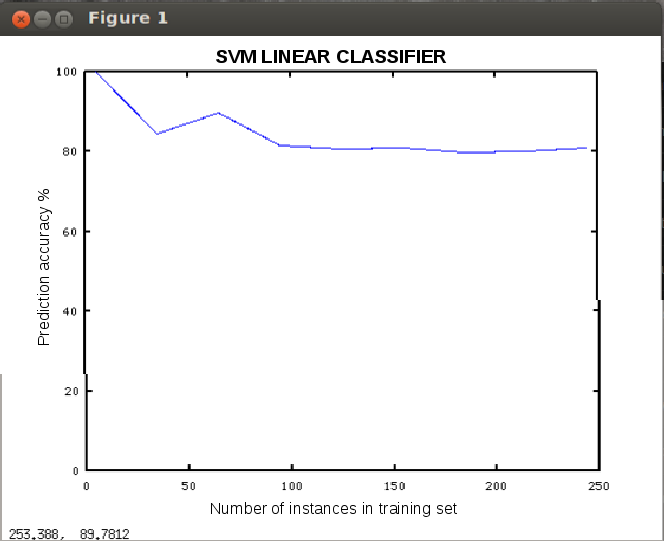
\includegraphics[width=2.5in, height=2.5in]{svml.png}
\caption{SVM(linear kernel) accuracy}
\end{figure}
Figure 2 above shows the prediction accuracy for a linear kernel SVM. It is immediately clear that the accuracy is lesser when compared to that produced by the Gaussian Kernel version of the SVM classifier. The reason for this is simple: The dataset is just no linearly seperable. i.e, there does not exist a straight line or a plane that perfectly seperates the dataset instances into two classes. Only a non-linear seperator (like the one produced by the Gaussian Kernel) can produce a good seperation of classes. Also, with a very few number of instances, the reported accuracy is close to 100\%. This is again because of the dataset idiosyncrasy as in the case of the Gaussian Kernel above. As the number of instances increases, the true accuracy of the classifier is revealed. Again, to keep execution time reasonable, the number of instances are increased in steps of 30 which explains the blockiness of the graph.

\begin{figure}
\centering
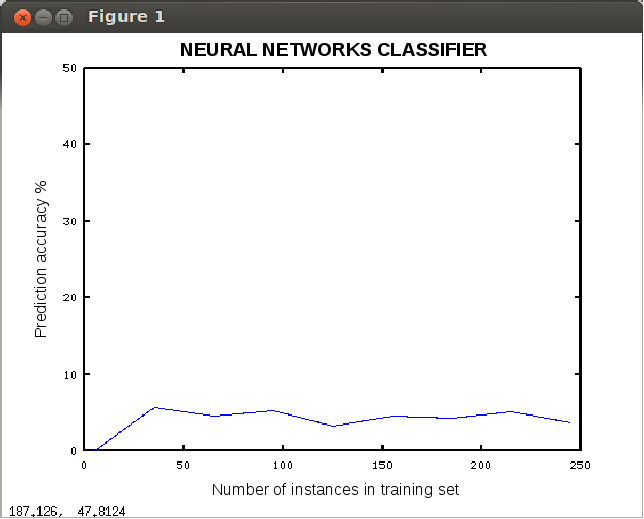
\includegraphics[width=2.5in, height=2.5in]{nn.png}
\caption{aNN(3 layer) accuracy}
\end{figure}
Figure 3 above shows the prediction accuracy for a NN classifier. Clearly, the accuracy is a whole lot inferior to those reported by any of the SVM classifiers above. The reason is that, the structure of the aNN is not fixed. It is decided by the programmer. We have gone with a NN structure with 3 stages, with the middle stage containing 50 neurons. The simple matter is, If you  get the structure of the NN right, you get good accuracy, you get the structure wrong, you can only expect below average accuracies. The upshot is that, the NN structure is decided by the programmer by intuition, which is not what we want in professional software programs. It is very difficult to come up with the right NN structure for the particular problem at hand. On the other hand, SVM implementation is free from such parameters that are decided by the programmer's intuition. The parameters of the SVM classifier are determined by the dataset and not by the programmer and thus easily adapts to different problems, unlike a NN implementation. This is not to say that, NN are always inferior. Several advanced NN strategies exist to overcome all the problems listed above, but with increased complexity.

\section{Applications}

Applications of Machine Learning and Data Mining in healthcare are only starting to appear in the real world. Machine Learning is still in its embryonic stages. Classifiers like the one we have implemented can be used by professional physicians to make an informed decision regarding the diagnosis of a patient, rather than just relying on intuition, to discover hidden information and patterns in the vast quantities of medical data available throughout the world, which is not possible by any human per se, because of the inability to make sense of such vast quantities of numerical data, as an aid to discover new relationships in the data that can provide the physician with previously unkown information about the patient's characteristics and thus enable him/her to provide the best possible care to the patient.  

As an example, consider that a cardiologist has details about a patient like race, sex, age, previous medical history etc. He/she can make use of the vast knowledge database provided by medical institutions around the world to make a diagnosis. Through software programs like ours the cardiologist can be provided with information such as races, age groups, patient sex and combinations of the previous that are more likely to have a heart disease. Previous medical history of the patient can be correlated with those of patients around the world and the accuracy of diagnosis on those patients can be considered while making a diagnosis for the current patient. Drugs prescribed and the outcome of those drugs are available in medical databases which can be used by software programs to provide sensible information regarding drugs that the patient is more likely to respond to in a positive manner.

\section{Future Improvements}

Our classifier only performs two class classification i.e, whether the results indicate a possible heart disease, or does not indicate any heart disease. Also the data used to make this classification only involves numerical data obtained directly by processing the SPECT heart images. Considering the above, we have the following areas in which the classifier can be improved in future versions.

Classification accuracy can further be improved by including the persons age, racial background, sex, pathophysiology, diet, air pollution in place of dwelling and previous medical history as features that aid the classification.  Such data though hard to obtain due to privacy issues can be a major accuracy booster. Such characteristics about patients can only be fully understood and made use of through a computer software that can crunch through vast quantities of data and provide the physician with easy-to-use, sensible information.

Another feature that has been debated for a long time in medical research is the demography in which the person has been brought up. It is obvious why this is so important. Take for example the fact that a malaria outbreak in America is more likely to reach pandemic proportions when compared to Africa or the fact that Africans are more suited to marathon running compared to Indians. To put it simply, it is just in their genes !!!.

Another simple improvement would be to provide a more fine-grained classification involving several classes of cardiac diseases instead of just a yes/no solution. Of course the training data should support such a classification by providig training instances for each of those classes. Using this allows us to abstain from making a very generalized prediction. We will be able to tell whether the patient suffers from Cardiomyopathy or Cardiac dysrhythmias or Endocarditis or Inflammatory cardiomegaly or Myocarditis or cerebrovascular disease or Peripheral arterial disease and many many more.  

\section{Acknowledgements}

Apart from our efforts, the success of this project depends largely on the encouragements and guidelines of many others. We take this opportunity to express our gratitude to the people who have been instrumental in the successful completion of this project.

We extend our deep regards to Dr. B.G Sangameshwara, Honorable principal of Sri Jayachamarajendra College of Engineering for providing an excellent environment for our education and his encouragement throughout our stay in college.

We would like to show our greatest appreciation to Professor and Head of the Department of Computer Science and Engineering Dr. C.N Ravikumar for his tremendous support and help and most importantly the time and opportunity to work on such a fulfilling project. Without his encouragement and guidance, this project would not have materialized. We would also like to sincerely thank our Project Guide and Professor Mrs. M.P Pushpalatha for her constant encouragement, valuable insight and her experienced suggestions.

Finally we would like to thank our friends for providing numerous insightful suggestions and our sincere thanks to all those who have contributed to this learning opportunity at every step of this project.

\newpage
%
% The following two commands are all you need in the
% initial runs of your .tex file to
% produce the bibliography for the citations in your paper.
\bibliographystyle{plain}
\bibliography{sigproc}  % sigproc.bib is the name of the Bibliography in this case
% You must have a proper ".bib" file
%  and remember to run:
% latex bibtex latex latex
% to resolve all references
%
\end{document}
